\begin{frame}{Headwall}

\begin{figure}
\centering

\begin{subfigure}{0.48\textwidth}
    \centering
    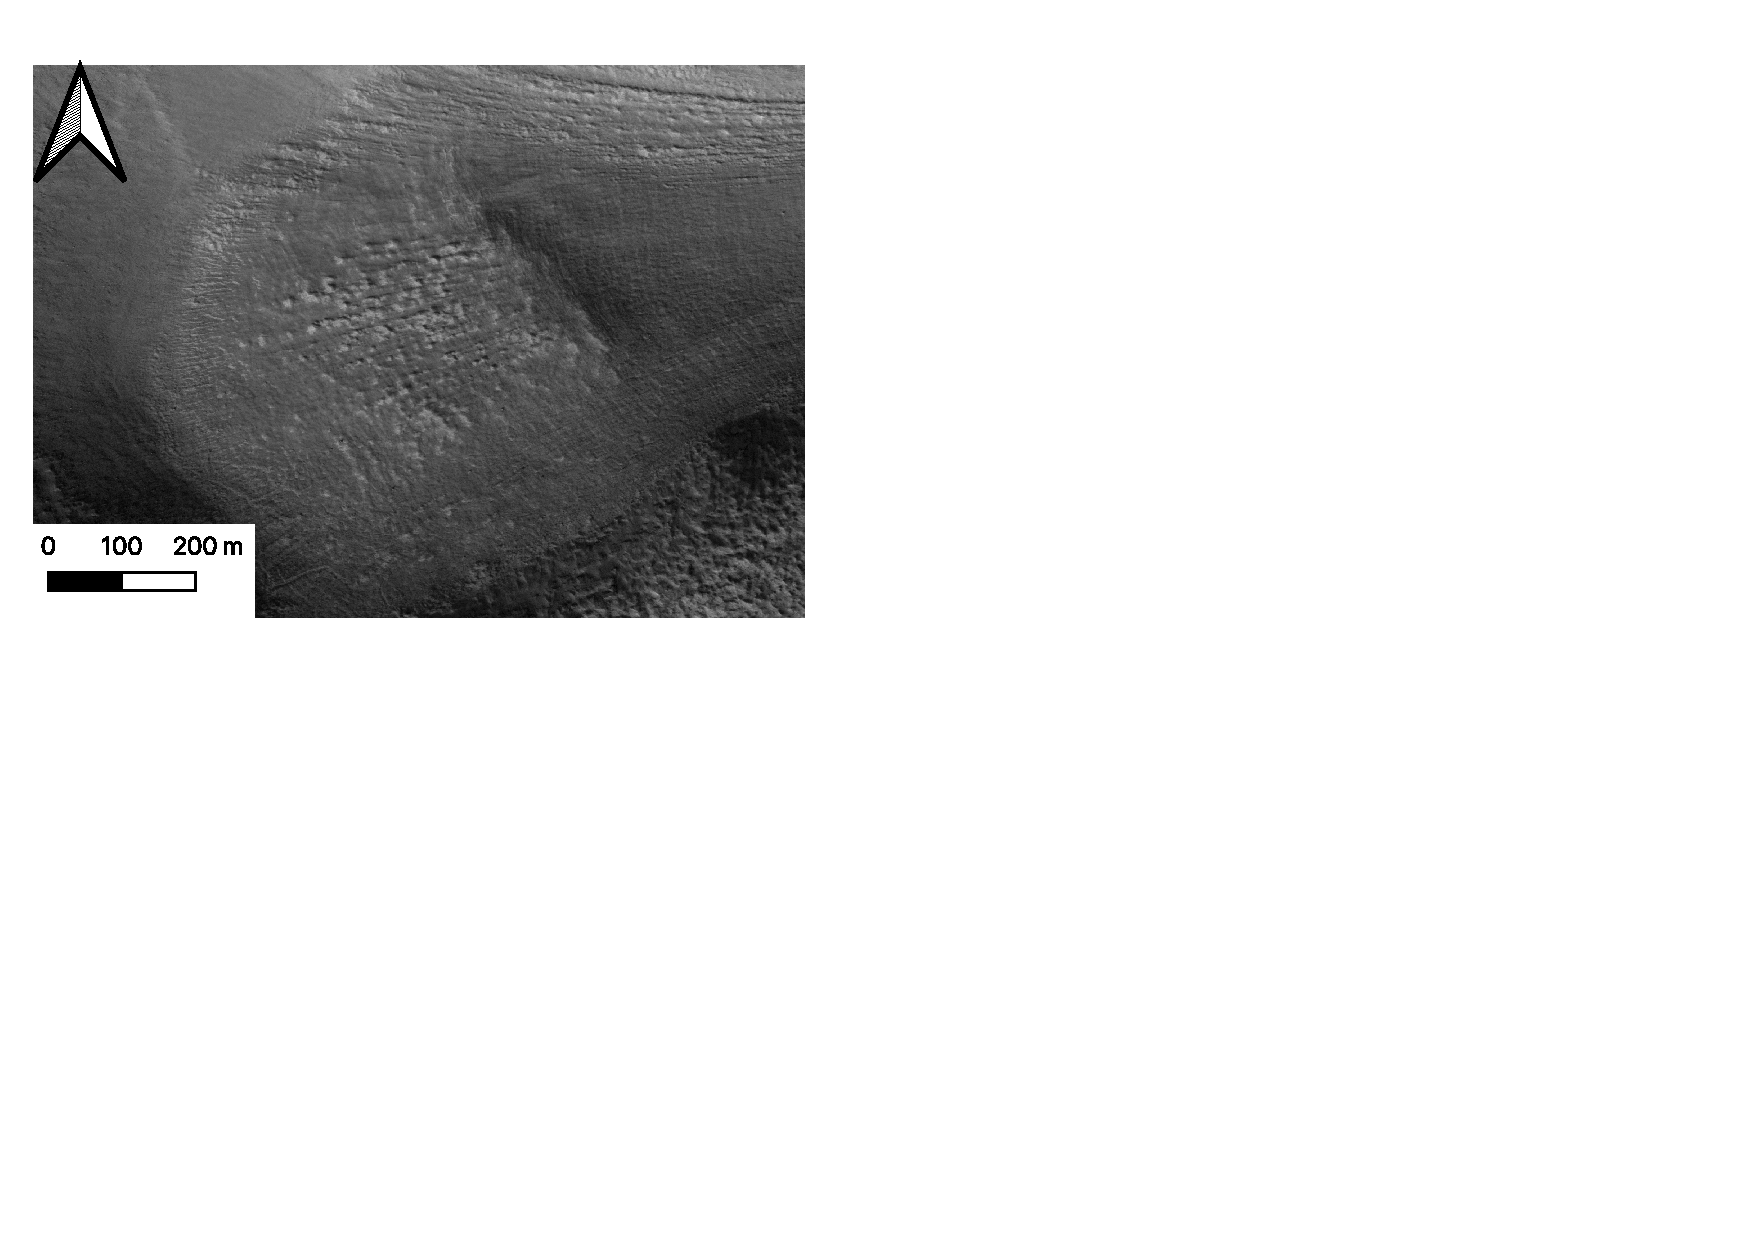
\includegraphics[
        width=\linewidth,
        height=0.65\textheight,
        keepaspectratio
    ]{Figures/HiRISE/Headwall_Img.pdf}
    \label{fig:Headwall_a}
\end{subfigure}
\hfill
\begin{subfigure}{0.48\textwidth}
    \centering
    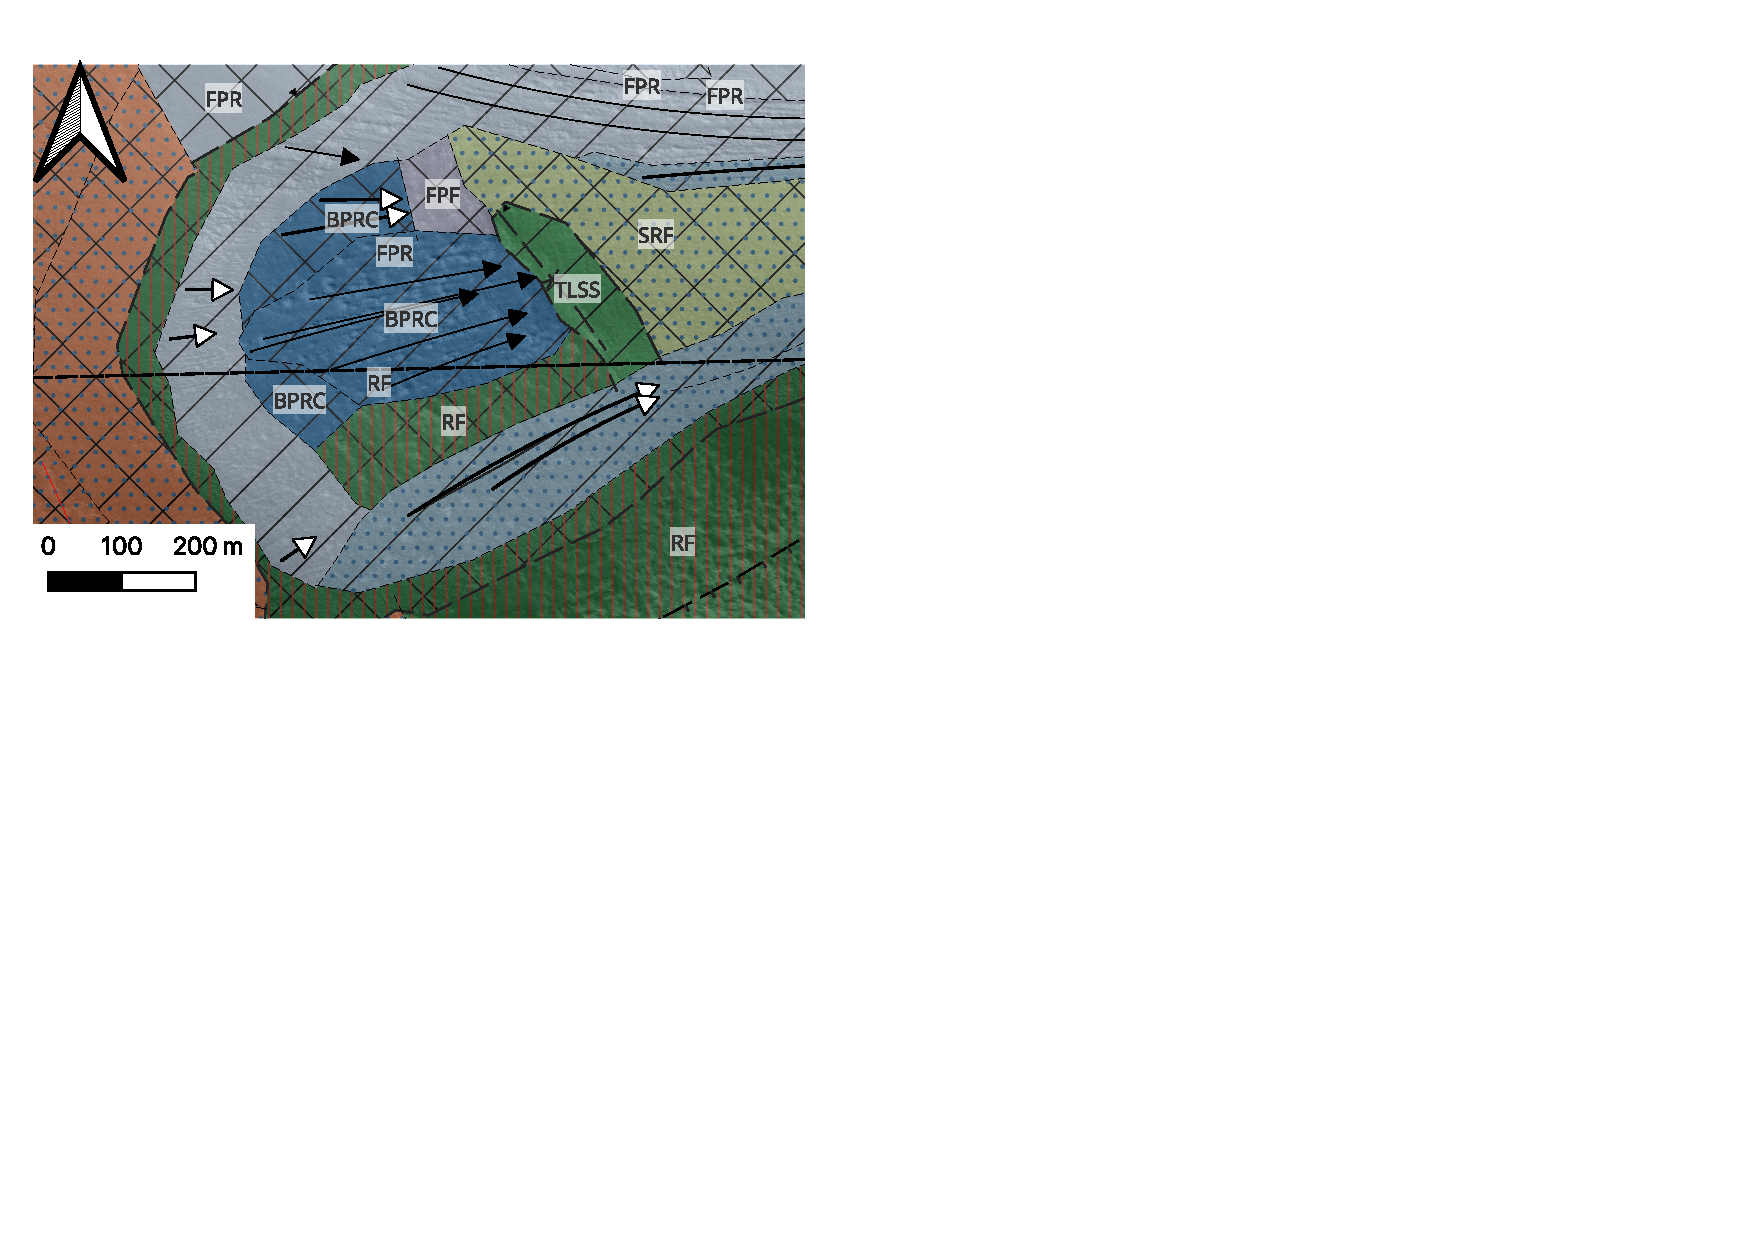
\includegraphics[
        width=\linewidth,
        height=0.65\textheight,
        keepaspectratio
    ]{Figures/HiRISE/Headwall_Map.pdf}
    \label{fig:Headwall_b}
\end{subfigure}

\caption{Headwall, showing linear flow features, rubble and a levee-type feature ($290 \mathrm{\ m} \times 95 \mathrm{\ m}$; centred at $34.62321^{\circ}$N, $16.79698^{\circ}$E) }
\label{fig:Headwall}

\end{figure}

\end{frame}
